% -------------------- 导言 -------------------- %
\documentclass[UTF8]{ctexart}

% 化学式
\usepackage[version=4]{mhchem}

\usepackage{lmodern}

% 设置页边距
\usepackage{geometry}
\geometry{left=3.18cm, right=3.18cm, top=2.54cm, bottom=2.54cm}

% 图片
\usepackage{graphicx}
% 并排
\usepackage{subfigure}
\usepackage{parskip}

% 页眉
\usepackage{fancyhdr}
\pagestyle{fancy}
\fancyhead[L]{\small \CJKfontspec{SimHei}第九届生物信息设计与技能竞赛}
\fancyhead[R]{\small \CJKfontspec{SimHei}大豆根系微生物的基因鉴定与基因功能预测}
\renewcommand{\headrulewidth}{1pt} % 分隔线宽度 1 磅

% 字体
% \usepackage{fontspec}
\setmainfont{Times New Roman} % 英文正文字体
% \setCJKmainfont{SimSun} % 中文正文字体
% \setCJKsansfont{SimHei}

% 设置标号深度
\setcounter{secnumdepth}{3}
\author{}
\date{}

\usepackage{caption}
\captionsetup[table]{
    font={small, bf},
    labelsep=quad,
    skip=0pt
}

\captionsetup[figure]{
    font={small, bf},
    labelsep=quad,
    skip=0pt
}

% 表格
\usepackage{booktabs}

\title{\vspace*{-1.5cm} \CJKfontspec{SimHei}大豆根系微生物的基因鉴定与基因功能预测}

% -------------------- 正文 -------------------- %
\begin{document}

    \maketitle\thispagestyle{fancy}
    \vspace*{-1.5cm}

    {\raggedleft
    {\zihao{5} \heiti  ——竞赛单元“2-1基因组”}}

    ~\\

    {\raggedleft
        团队名称:水哥微生物小队\\
        指导老师:郑金水\\
        团队成员:张敦彪,张子栋,颜旭,姚代洪\\}
    
    ~\\

    {\raggedright
    {\zihao{4} \heiti 摘要}}

    高通量培养与鉴定\textsuperscript{\cite{ref1}}可用于从给定环境和植物物种的本地根微生物组样本中建立一个分类学上全面的细菌培养收集,通过 16S rRNA基因扩增子测序对根样品的细菌多样性进行评价,筛选出具有相应16S rRNA 基因序列的培养菌。通过对大豆根系微生物的高通量培养筛选可以鉴定其基因的类型,进而对其基因功能进行预测。
    
    ~\\

    {\heiti \zihao{-4} \raggedright 关键字:} {\zihao{5} 高通量培养,基因鉴定,功能预测}

    
    % % 目录设为页码 0(从正文起为第一页)
    % \setcounter{page}{0}

    % % 目录的页脚设为空
    % \thispagestyle{empty}


    % \chapter{Hello}

    \section{引言}

    \subsection{根系微生物群}

    根系微生物是指生活在植物根系附近的微生物群落,包括细菌、真菌和古菌等。它们与植物根系形成一种共生关系,相互作用并互利共生。根系微生物可以对植物生长和健康产生积极影响。研究根系微生物对于促进植物生长健康、提高作物产量质量、维护土壤生态系统健康以及发掘新的生物资源具有重要意义。
    
    传统的微生物培养方法是基于单个菌落的分离和培养,但是由于绝大部分微生物无法在常规培养条件下生长,很多微生物资源依然无法被发现和利用。高通量培养是一种用于微生物的培养和筛选的技术,通过该技术可以大大提高微生物的培养效率和筛选速度,同时也有助于扩展微生物资源库,挖掘未知微生物代谢产物等领域的研究。而高通量培养可以利用微型板或微流控芯片等设备将微生物单个分离后进行多重并行培养,以大幅提高微生物的培养效率。此外,高通量培养还可以借助自动化解决方案,实现对大量微生物的快速筛选。

    本文从新鲜大豆根系(根际、根内)中高通量分离培养细菌,使用梯度稀释的方法增加获得单一细菌的比例,采用双侧标签PCR扩增法高通量鉴定分离培养细菌的 16S rRNA 基因。同时开发了一套从二代测序下机数据到基因鉴定个基因功能分析的全套流程。

    \section{材料与方法}

    \subsection{培养基的制作}

    实验中需要三种不同的培养基(三种培养基均高压蒸汽灭菌):

    \begin{table}[htb]
        \centering
        \caption{实验所需培养基}
        \begin{tabular}{cc}
            \toprule
            培养基类型 & 配置方法\\
            \midrule
            TSB 培养基 & $\mathrm{30~g/L}$ TSB,蒸馏水定容\\
            10\% TSB培养基 & TSB 培养基按照体积分数 10\% 进行稀释\\
            10\% TSB培养基+丙酮酸钠 & $\mathrm{30~g/L}$ TSB,$\mathrm{10~mM/L} $丙酮酸钠,蒸馏水定容\\
            \bottomrule
        \end{tabular}
    \end{table}

    \subsection{大豆根系菌群的获取}

    在华中农业大学 BMB 课题组大豆孢囊线虫大棚中摘取自然条件下生长、表型正常的未开花的大豆,在取样前不宜过多浇水,以免造成大豆根系附着较多土壤,不易除去。用手轻轻拨去大豆根系的土壤以去除大量土壤团聚体,此后将大豆根系置于手掌虎口处轻轻抖动,去除碎土。

    \begin{figure}
        \centering
        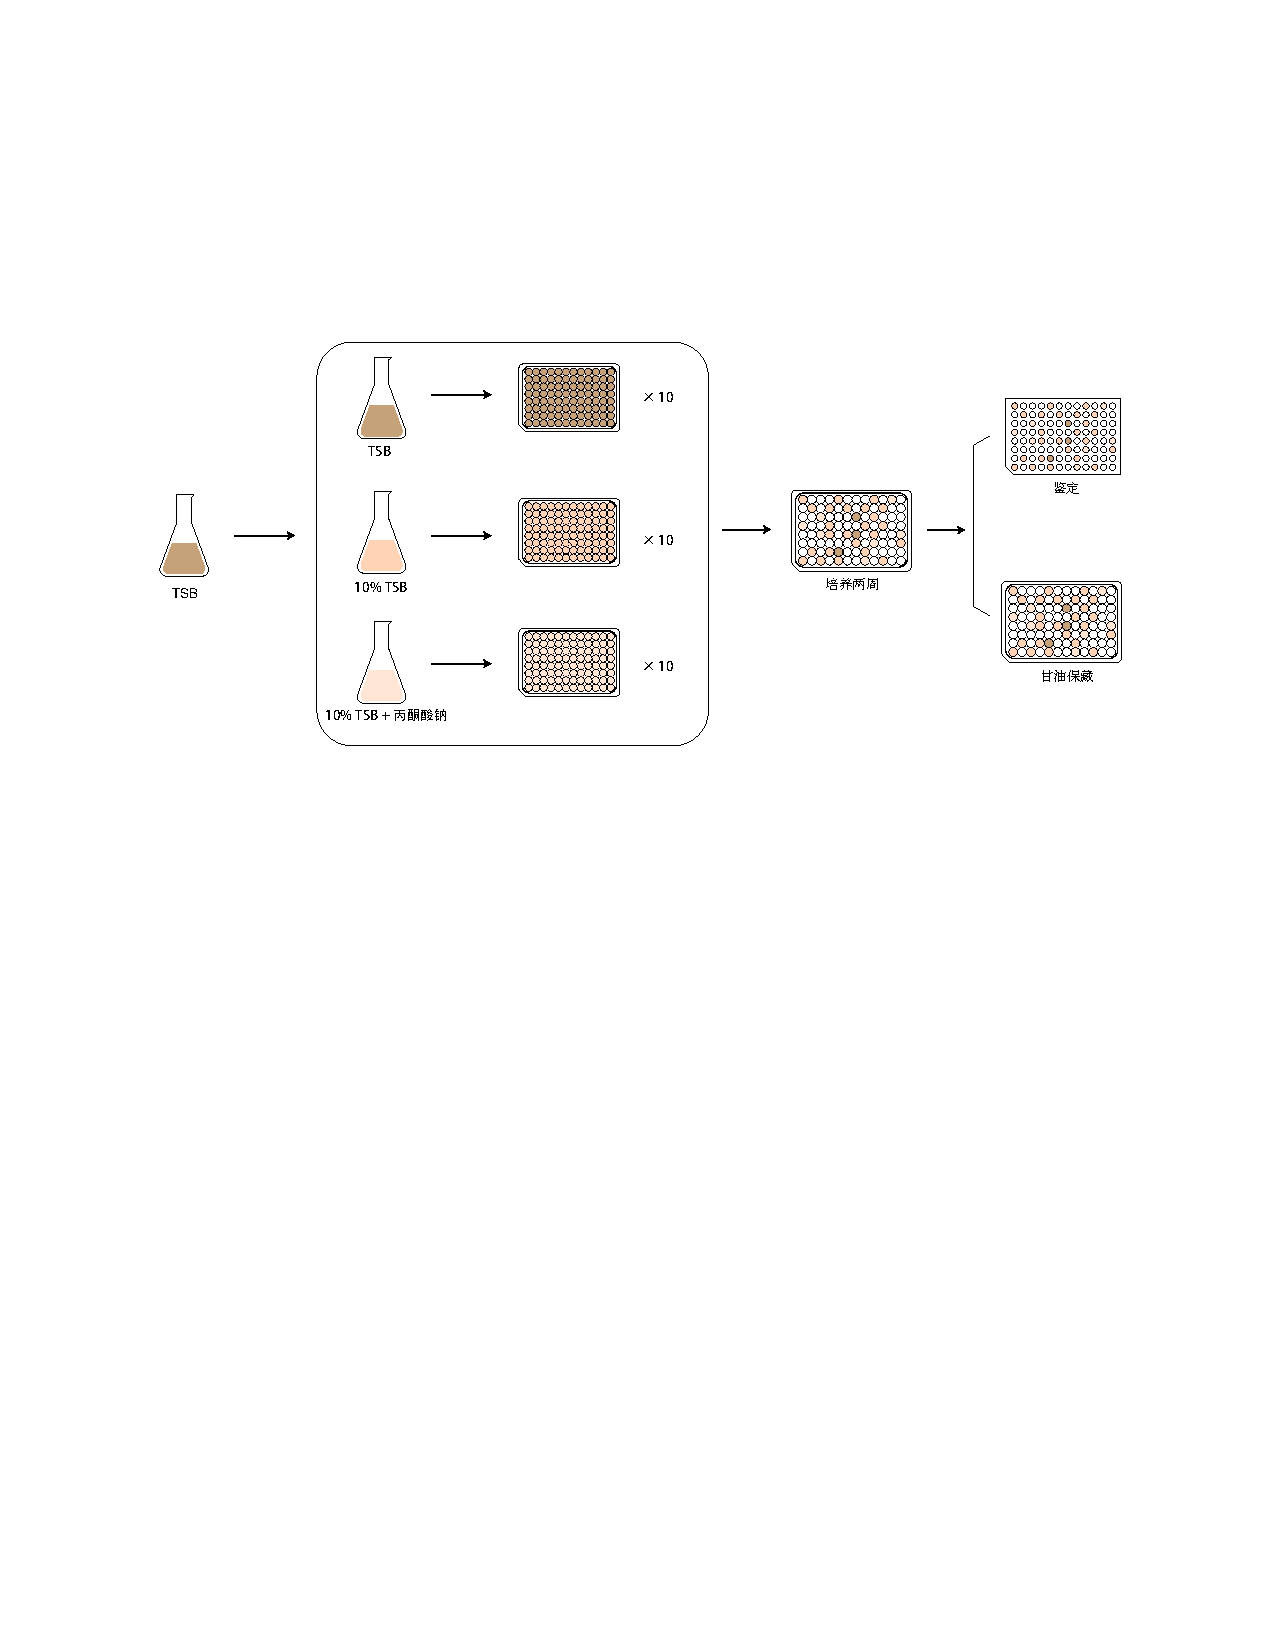
\includegraphics[width=\textwidth]{img/CulturePipeline.pdf}
        \caption{高通量培养流程}
    \end{figure}

    \subsubsection{根际样本}
        超净工作台中将大豆根系置于无菌滤纸上,使用无菌刀片截取其下方约3cm的根系,总共截取3g的大豆根系样本。拿取 $\mathrm{10x~PBS}$ 溶液,按照体积分数的 10\% 稀释为 $\mathrm{1x~ PBS}$ 溶液约 100~mL 置于两个 50~mL 的离心管中。将截取的根系样本置于 50~mL 的 $\mathrm{1x~ PBS}$ 溶液中来回水平摇匀,将其以 1800~rpm 的速度震荡 20~min,取出其中的根系,将溶液过500目筛,获得根际样本。

    \subsubsection{根内样本}
        按照上述方法新截取约 3~g 的大豆根系,使用无菌水持续冲洗,直至除去所有的土壤颗粒。将根系转移至一个新的含有 50~mL 的 1x~PBS 溶液的离心管中,以 1800~rpm 的速度震荡处理 20~min,从离心管中取出根系,使用无菌滤纸吸干,从根表面除去 PBS 溶液,使用无菌水冲洗三次,将根系置于含有 50~mL 无菌水的离心管中,进行超声处理 5~min,将根系取出置于含有 50~mL 的75\%体积分数的酒精溶液的离心管中,震荡 1~min,取出根系,使用无菌水冲洗三次,将根系悬浮在 50~mL 的 10~mmol/L 的无菌$\ce{MgCl2}$溶液中,使用无菌研钵研碎根系直至其均匀,将研钵内液体过 500 目筛获取根内样本\textsuperscript{\cite{ref2}}。

        根内样本与根际样本均置于 4℃ 储存。

    \subsection{分液与流式细胞分选}

    用分液仪将液体培养基分装到 60 个 384 孔板,再用流式细胞分选仪将根际与根内样本转移到每个孔中并做好标记。

    \subsection{高通量培养}
    高通量培养是一种用于快速筛选和培养大量微生物的方法。它利用自动化设备和高效的培养技术,可以同时处理多个微生物样品,并快速判断微生物的生长状况和特性。本实验中通过流式细胞分选仪连续地将多个样本注入仪器中进行分析和分选,从而实现快速、连续地处理大量样本,提高分选效率。对比需要一个月时间传统的分菌方法\textsuperscript,高通量培养只需要一天的时间便可完成。

    \subsection{PCR 扩增与电泳鉴定}
        将得到的 PCR 管每个孔中按表 2 比例配置反应体系,按照对应程序将 PCR 管放入 PCR 仪按照表 3 程序进行扩增。

    \begin{table}[!htb]
        \begin{minipage}[h]{0.4\linewidth}
            \centering
                \caption{PCR 反应体系}
                \begin{tabular}{cc}
                    \toprule
                    成分        & 体积(μL)\\
                    \midrule
                    F 引物      & 1\\
                    R 引物      & 1\\
                    \ce{ddH2O}  & 7\\
                    Mix         & 10\\
                    原样液      & 1\\
                    \bottomrule
                \end{tabular}
        \end{minipage}
        \begin{minipage}[h]{0.6\linewidth}
            \centering
                \caption{PCR 程序设定}
                \begin{tabular}{cccc}
                    \toprule
                    循环数  & 流程 & 温度 & 时间\\
                    \midrule
                    1 & 预变性 & 98℃ & 10~min\\
                    & 变性 & 95℃ & 30~s\\
                    2-36 & 复性 & 55℃ & 30~s\\
                    & 延伸 & 72℃ & 90~s\\
                    37 & 终延伸 & 72℃ & 5~min\\
                    \bottomrule
                \end{tabular}
        \end{minipage}
    \end{table}

    实验采上下游 PCR 引物设计,下游引物是针对目标基因(或序列)末端的引物,而上游引物则与目标基因(或序列)起始点相匹配。用 F 与 R 引物测定了培养菌全长的 16S rRNA 基因序列。

    通过 PCR 后的产物电泳结果与 DNA Marker 进行对比来检验 PCR 产物是否合格。

    \subsection{产物回收与浓度测定}
    \subsubsection{产物回收}
    短暂离心 PCR 产物后用移液枪测体积,并转移至灭菌的 2~mL 离心管中,加入 Buffer DP,混匀 15~S 后加入加入 2.5 倍体积 Buffer DP 和 1 倍体积异丙醇,离心收集管壁液滴。将 HiPure 柱子套在收集管中,混合液转移至柱子,$\mathrm{10000\times g}$ 离心 60~s,重复上述步骤5-6次直到混合体积小于 700~μL 后倒掉滤液。柱子套到回收管中,加入 500~μL Buffer DW2,$\mathrm{10000\times g}$ 离心 60~s 后倒掉滤液,套在回收等中,$\mathrm{10000\times g}$ 离心 2~min。将柱子套在 2~mL 的离心管中,加入 25~μL Elution Buff 至柱子的膜中央,静置 1~min 后 $\mathrm{10000\times g}$ 离心 1~min,最后得到产物。

    \subsubsection{浓度测定}
    使用微量分光光度计来测定得到产物的浓度。

    \subsection{测序}
    为了让来自不同板的菌体的DNA总量大概一致,按浓度混合后再送往测序公司进行测序。

    \subsection{16S rRNA 分析}
    16S rRNA 序列由高度保守的不可变区和相对可变的可变区组成,不可变区域是 16S rRNA 序列中相对较短的区域,其在细菌和古菌中高度保守,即基本保持相同的序列。
    
    16S rRNA 是一个长序列,经过多年的研究和数据库的积累,已经建立了广泛和全球性的 16S rRNA 数据库\textsuperscript{\cite{ref3}}。这些数据库中包含了大量的细菌和古菌的 16S rRNA 序列,使得通过比对新测序的 16S rRNA 序列与数据库中的序列进行比较成为可能。通过将新测序的 16S rRNA 序列与数据库中已知的序列进行比对,可以根据比对结果确定其与已知物种或菌株的相似性,并进一步进行物种或菌株的鉴定。

    \subsection{扩增子分析}
    培养组流程\textsuperscript{\cite{ref4}}采用 Shell/R/Perl 语言编写脚本,整合了微生物组分析常用软件 QIIME、\\VSEARCH、GraPhlAn 等,定制完成的高通量培养物鉴定流程,可实现双端标签化扩增子文库的分析和可视化全流程。

    \subsubsection{质量分析}
    使用 FastQC 进行质量分析。测序结果较好,均符合预期。

    结果保存至 \verb| result\fastqc.test\BeanRoot_fastqc.html |。

    \subsubsection{数据预处理}
    在使用 QIMME2 之前,要先使用 R 手动编写并导出符合 QIMME2 要求\textsuperscript{\cite{ref5}}的 Metadata mapping file。由于二代测序下机数据为双端测序序列,在开始数据分析之前,需要使用 VSEARCH 进行双端测序合并。然后从序列中拆分出用于识别菌孔的 Barcode 和引物,得到扩增子。随后利用拆分的 Barcode 与 Mapping file 将序列重命名为板和孔的位置。

    同时我们也完成了对每板每孔数据读长、读长数量的统计(如图 2)。

    \begin{figure}[htbp]
        \centering
        \subfigure[根内样本测序读长分布]{
            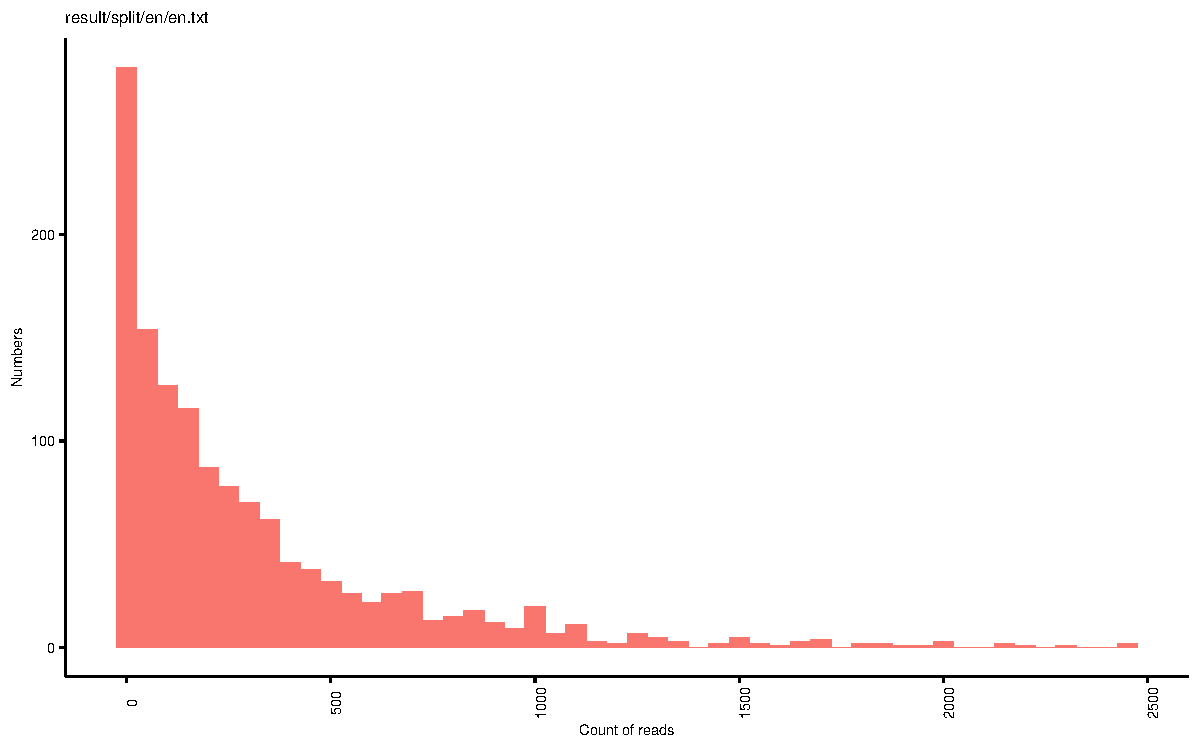
\includegraphics[width=0.48\textwidth]{img/en.txt.histogram.pdf}
        }
        \subfigure[根际样本测序读长分布]{
	        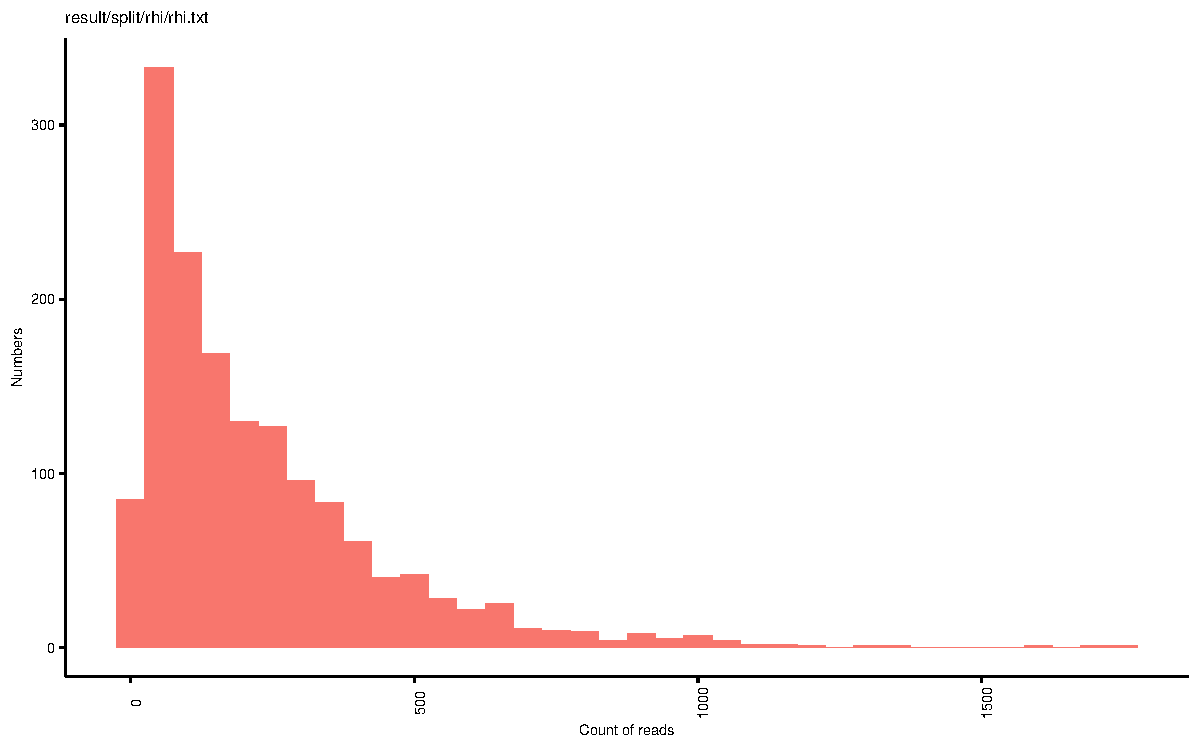
\includegraphics[width=0.48\textwidth]{img/rhi.txt.histogram.pdf}
        }
        \\
        \subfigure[根内样本测序读长分布]{
            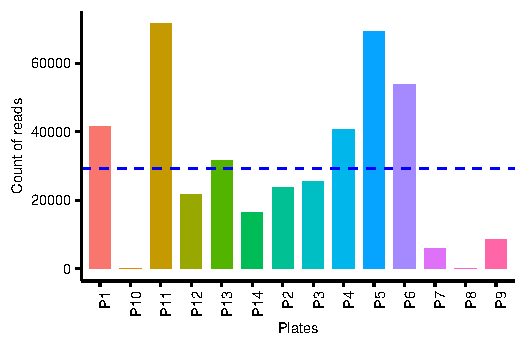
\includegraphics[width=0.48\textwidth]{img/en.txt.plate.pdf}
        }
        \subfigure[根际每板读长数量]{
            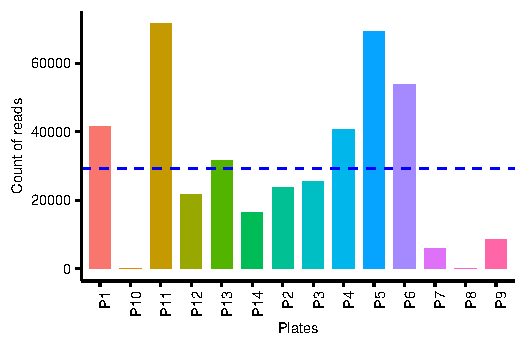
\includegraphics[width=0.48\textwidth]{img/en.txt.plate.pdf}
        }
            \caption{测序读长分布}
    \end{figure}

        % \centering
        % \begin{minipage}[t]{0.48\textwidth}
        %     \centering
        %     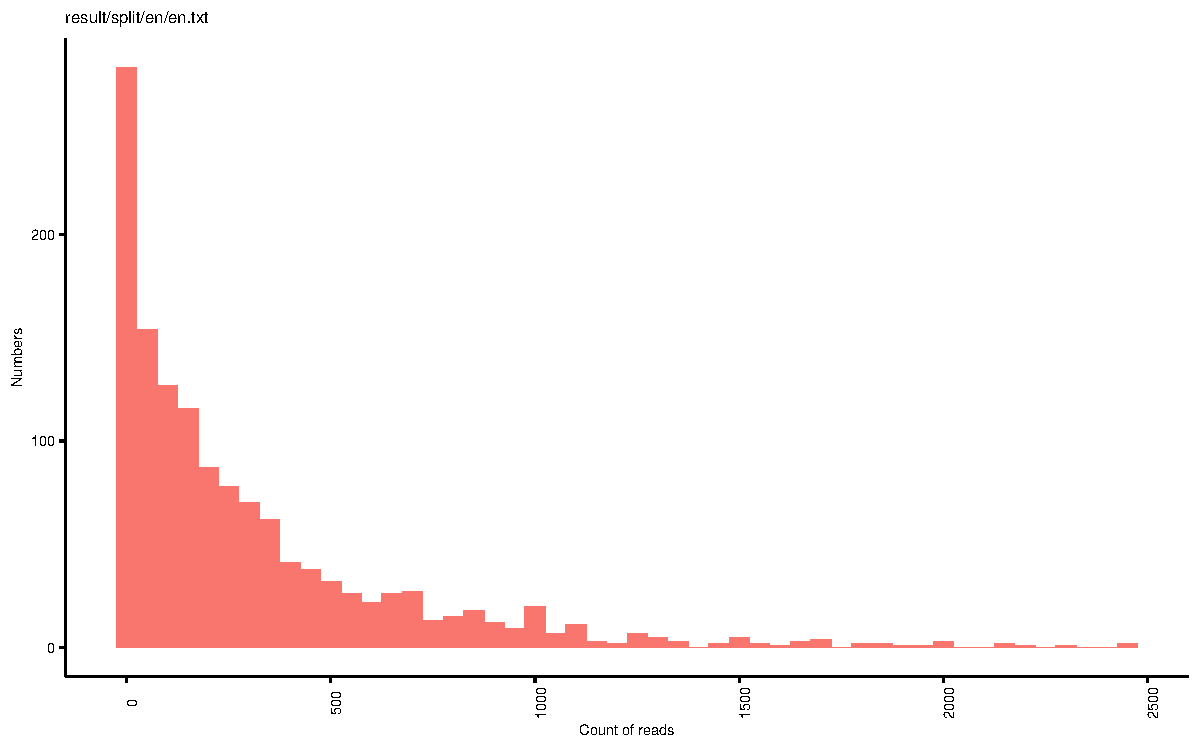
\includegraphics[width=6cm]{img/en.txt.histogram.pdf}
        %     \caption{根内样本测序读长分布}
        % \end{minipage}

        % \begin{minipage}[t]{0.48\textwidth}
        %     \centering
        %     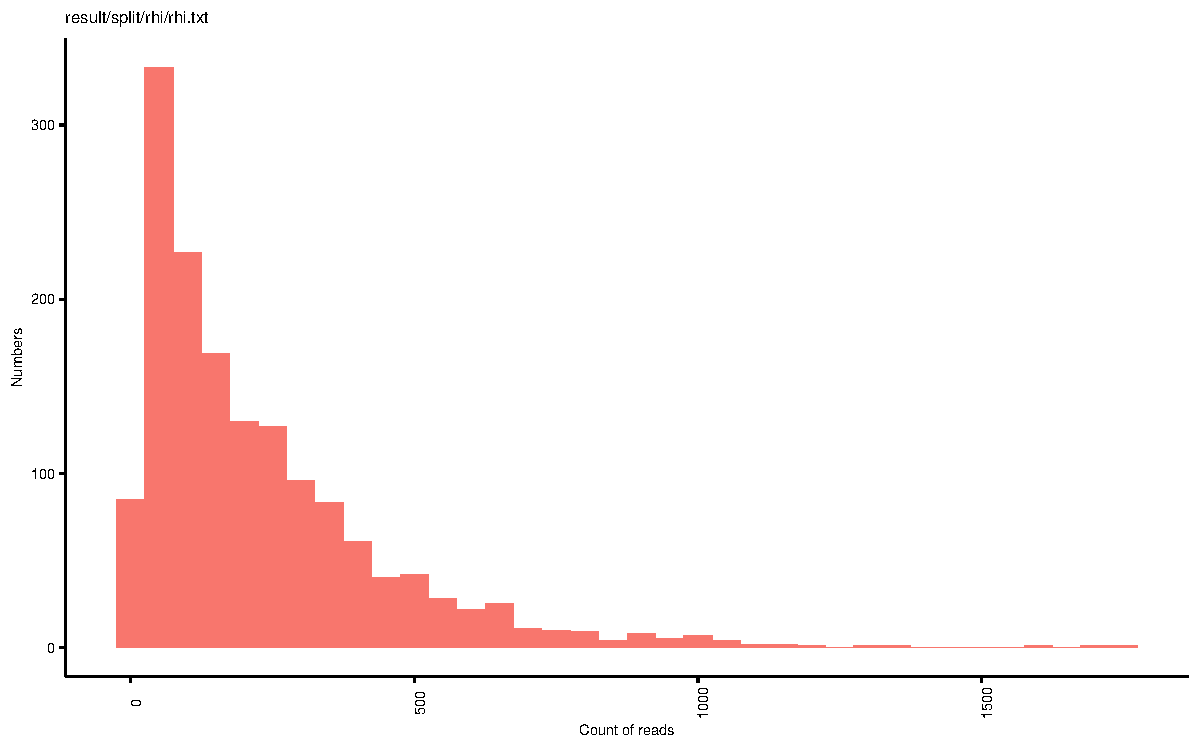
\includegraphics[width=6cm]{img/rhi.txt.histogram.pdf}
        %     \caption{根际样本测序读长分布}
        % \end{minipage}\\
         
        % \centering
        % \begin{minipage}[t]{0.48\textwidth}
        %     \centering
        %     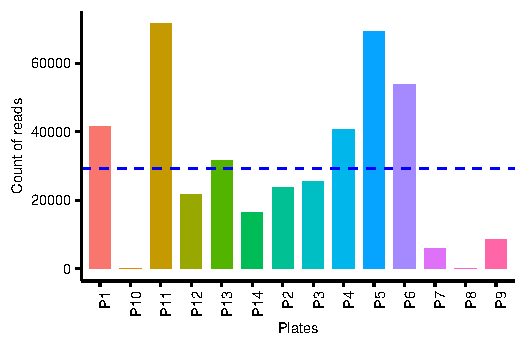
\includegraphics[width=6cm]{img/en.txt.plate.pdf}
        %     \caption{根内每板读长数量}
        % \end{minipage}

        % \begin{minipage}[t]{0.48\textwidth}
        %     \centering
        %     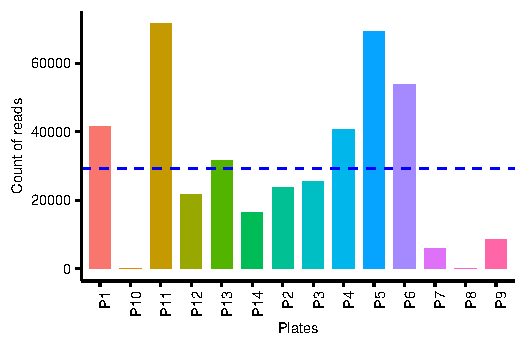
\includegraphics[width=6cm]{img/en.txt.plate.pdf}
        %     \caption{根际每板读长数量}
        % \end{minipage}\\

    % {\zihao{4} \heiti \raggedleft 参考文献}

    \begin{thebibliography}{99}
        \bibitem{ref1} Jingying Z,Xin Y L,Xiaoxuan G, et al. High-throughput cultivation and identification of bacteria from the plant root microbiota[J]. Nature Protocols,2021,16(2). https://doi.org/10.1038/s41596-020-00444-7

        \bibitem{ref2} 李亭玉,李太元.益生菌发酵工艺中蜡样芽孢杆菌的分离鉴定[J].当代畜禽养殖业, 2019(6):2. CNKI:SUN:DAYZ.0.2019-06-006.
 
        \bibitem{ref3} Nadav B,Grant G,H C W, et al. Genome-wide prediction of disease variant effects with a deep protein language model.[J]. Nature genetics,2023. https://doi.org/10.1038/s41588-023-01465-0

        \bibitem{ref4} Jingying Zhang, Yong-Xin Liu, Xiaoxuan Guo, Yuan Qin, Ruben Garrido-Oter, Paul Schulze-Lefert, Yang Bai. 2021. High-throughput cultivation  and identification of bacteria from the plant root microbiota. Nature Protocols 16: 988-1012. https://doi.org/10.1038/s41596-020-00444-7

        \bibitem{ref5} Douglas, G.M., Maffei, V.J., Zaneveld, J.R. et al. PICRUSt2 for prediction of metagenome functions. Nat Biotechnol 38, 685–688 (2020). https://doi.org/10.1038/s41587-020-0548-6

        \bibitem{ref6} Chen Yang and others. (2023). ggpicrust2: an R package for PICRUSt2 predicted functional profile analysis and visualization. Bioinformatics, btad470. https://doi.org/10.1093/bioinformatics/btad470

        \bibitem{}
        % http://qiime.org/documentation/file_formats.html ;访问于 2023 年 9 月
    \end{thebibliography}

\end{document}